%!TEX root = ../../sbc-template.tex

%conceito, inspiração biológica
As \emph{Redes Neurais Artificiais} (RNAs) são um modelo de computação caracterizado por sistemas que, em algum nível, lembram a estrutura do cérebro humano. São sistemas paralelos e distribuídos, compostos por unidades de processamento simples, os \emph{neurônios artificiais}, que calculam funções matemáticas, normalmente não-lineares. Estes neurônios são dispostos em uma ou mais camadas e interligados por um grande número de conexões normalmente unidirecionais e comumente associadas a pesos, que armazenam o conhecimento representado no modelo e ponderam a entrada recebida por cada neurônio da rede. Os principais atrativos das RNAs envolvem a capacidade de capturar tendências a partir de um conjunto de exemplos e dar respostas coerentes para dados não-conhecidos, ou seja, de generalizar a informação aprendida \cite{Teresa:Livro}.

A motivação para a criação deste modelo vem do funcionamento do cérebro biológico, que é formado por neurônios interligados e que se comunicam entre si de modo contínuo e paralelo através de impulsos nervosos. Esta complexa rede neural biológica é capaz de reconhecer padrões e relacioná-los, produzir emoções, pensamentos, percepcção e cognição. Cada neurônio biológico é composto de um corpo, dendritos e um axônio, como ilustrado na Figura \ref{fig:neuronio_biologico}. Os dendritos são responspaveis pela recepção de impulsos nervosos vindos de outros neurônios; o corpo combina os sinais recebidos pelos dendritos e caso o resultado ultrapasse determinado limiar de excitação do neurônio, são gerados novos impulsos nervosos, que são transmitidos pelo axônio até os dendritos dos neurônios seguintes. Esta conexão unilateral entre neurônios biológicos, denominada sinapse, encontra-se ilustrada na Figura \ref{fig:redeneuralbiologica}.

\begin{figure}
	\caption{Redes neurais biológicas. Fonte: FALTANDO!}
	\begin{subfigure}[h]{0.5\linewidth}
		\caption{Neurônio biológico e seus componentes.}
		\label{fig:neuronio_biologico}
		\includegraphics[width=0.7\linewidth]{img/neuronio}
	\end{subfigure}
	\begin{subfigure}[h]{0.5\linewidth}
		\caption{Sinapse entre neurônios.}
		\label{fig:redeneuralbiologica}
		\includegraphics[width=\linewidth]{./img/redeneuralbiologica.jpg}
	\end{subfigure}%
\end{figure}


Com base no modelo biológico, McCulloch e Pitts propuseram em  um neurônio artificial \cite{mcculloch1943logical}. Como mostrado na Figura \ref{fig:neuronio}, o modelo de McCulloch e Pitts de neurônio artificial contém $n$ terminais de entrada, denotados por $x = x_1, \ldots, x_n$, e um terminal de saída $y$. Esta organização faz uma alusão aos dendritos, centro e axônio de um neurônio biológico. A saída é mapeada por uma função $y = \sigma(z)$, expressa na Equação \ref{eq:funcao_neuronio}, em que a soma ponderada $z$ do vetor de entrada $x$ pelo conjunto de pesos $w = w_1, \ldots, w_n$
deve ser submetida a uma função de ativação $\sigma$, que determina se aquele neurônio é ativado ou não, no sentido de ter \todo{definir ativação de um neurônio e colcoar a citação aqui}. No caso de um neurônio mais simples como o de McCulloch e Pitts, a função de ativação consiste de verificar se a soma ponderada $z$ é maior ou igual a um limiar de ativação $\theta$, conforme a Equação \ref{eq:ativacao_limiar} \cite{mcculloch1943logical}. Atualmente, a escolha da função de ativação $g(\cdot)$ das camadas ocultas e da camada de saída deve considerar funções contínuas e deriváveis \cite{hornik1991approximation}, em que comumente são optadas pelas funções apresentadas na Tabela  \ref{tab:ativacoes}.

\begin{figure}[ht]
	\centering
	\includegraphics[width=0.7\textwidth]{img/perceptron.png}
	\caption{Representação de um neurônio}
	\label{fig:neuronio}
\end{figure}

\begin{gather}\label{eq:funcao_neuronio}
	z = \sum_{i=1}^n x_i w_i + b_i\\
	y = \sigma(z)
\end{gather}

\begin{equation}\label{eq:ativacao_limiar}
	y = \sigma(z) =
		\begin{cases}
			0, & \text{se } z < \theta\\
			1, & \text{se } z \geq \theta
		\end{cases}
\end{equation}

%!TEX root = ../main.tex

\begin{table}[H]
	\scalefont{0.8}
	\centering
	\label{tab:ativacoes}
	\begin{adjustbox}{width=0.7\textwidth}
		\begin{tabular}{l l p{6.5cm} l}
			\toprule
			Nome 			 		& Gráfico & Equação & Intervalo\\
			\midrule
			Identidade ou Linear		&
			 	\Centerstack{\includegraphics[width=0.15\textwidth]{img/identidade}}
			&
				$
					\begin{aligned}
						\sigma(z) = z
					\end{aligned}
				$
				& $(-\infty, + \infty) $\\
			\hline
			Tangente Hiperbólica		&
				\Centerstack{\includegraphics[width=0.15\textwidth]{img/tanh}}
				&
				$
					\begin{aligned}
						\sigma(z) = tanh(z) =\frac{(e^z - e^{-z})}{(e^z + e^{-z})}
					\end{aligned}
				$
				 & $(-1,1)$\\
			\hline
			Sigmoide ou Logística		&
				\Centerstack{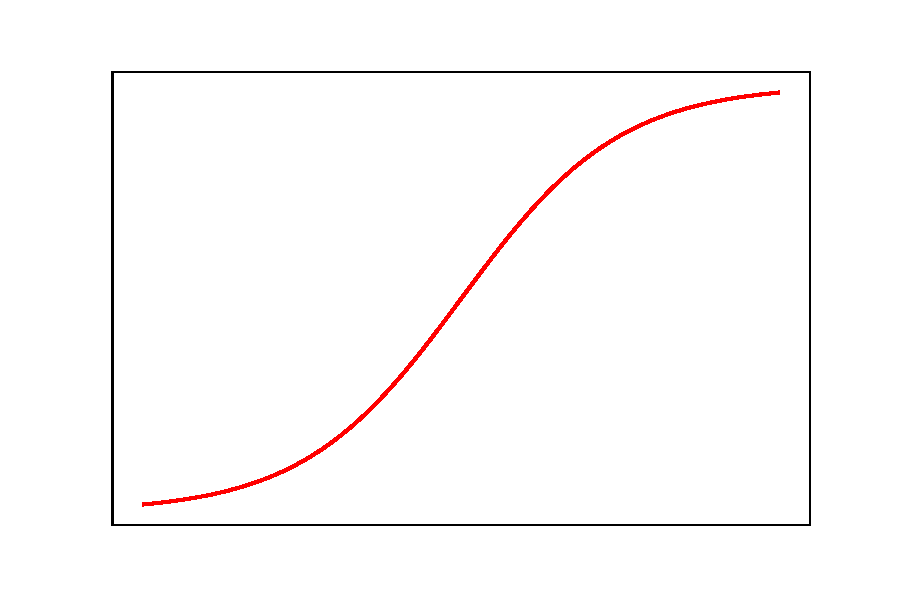
\includegraphics[width=0.15\textwidth]{img/sigmoid}}
				&
				$
					\begin{aligned}
						\sigma(z) = \frac{1}{1+e^{-x}}
					\end{aligned}
				$
				& $ (0,1) $\\
			\hline
			Unidade Linear Retificada	&
				\Centerstack{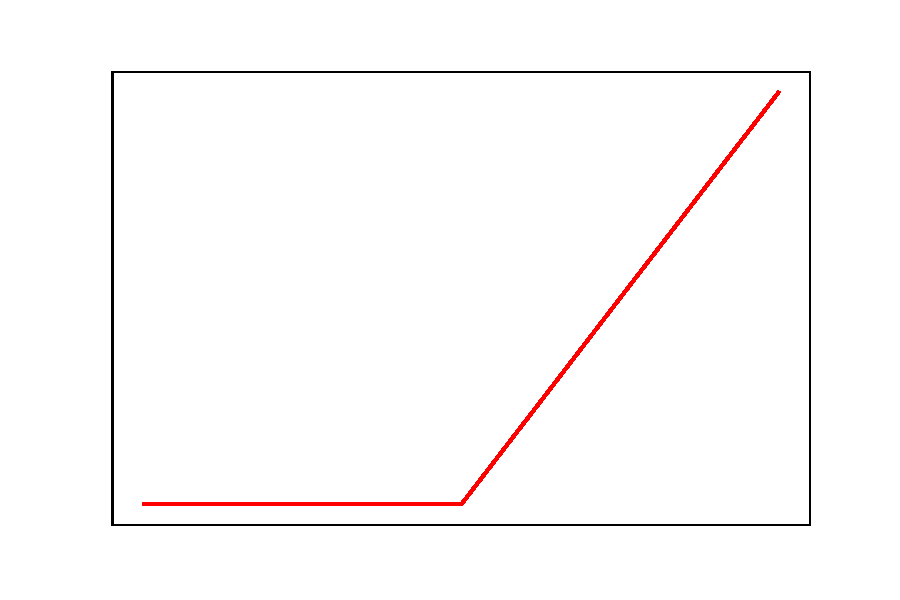
\includegraphics[width=0.15\textwidth]{img/relu}}
				&
				$
					\begin{aligned}
						\sigma(z) = max(0,z)
					\end{aligned}
				$
				& $ [0, \infty) $\\
			\hline
			Softmax					&
				\Centerstack{\includegraphics[width=0.15\textwidth]{img/softmax}}
				&
				$
					\begin{aligned}
						g(z_j) = \frac{e^{z_j}}{\sum^K_{j=1} e^{z_k}} \hspace{0.2cm}j=1, \ldots, K
					\end{aligned}
				$
				& $(-\infty, \infty)$\\
			\bottomrule
		\end{tabular}
	\end{adjustbox}
	\caption{Exemplos de funções de ativação}
\end{table}


Em 1958, Frank Rosenblatt desenvolveu o neurônio \emph{Perceptron} \cite{rosenblatt1958perceptron}, que mais tarde seria empregado como a unidade de processamento das RNA e de outros modelos de ML, a exemplo das \emph{support vector machines}. O Perceptron de Rosenblatt agregou ao neurônio de McCulloch e Pitts conceitos cruciais para a caracterização das RNAs como são conhecidas hoje, como a não obrigatoriedade de igualdade dos pesos e limiares de ativação, a possibilidade de os pesos serem positivos ou negativos, a diversidade de funções de ativação, entre outros. Além desta caracterização, uma contribuição relevante deste trabalho contempla a proposição de um algoritmo de aprendizado que permite a adaptação dos pesos de uma RNA através da otimização do desempenho da rede. Isto atribuiu ao modelo Perceptron a capacidade de aprender tarefas que contenham dados linearmente separáveis \cite{Teresa:Livro}.

Este modelo inicial apresentava algumas limitações, atribuídas principalmente à sua linearidade e simplicidade, características que possibilitam resolver apenas problemas linearmente separáveis \cite{Teresa:Livro}. A disposição de neurônios em camadas e a utilização de funções de ativação nas saídas dos neurônios caracterizou as RNAs, capazes de serem aproximadas universiais de qualquer função contínua graças à otimização por minimização da dissimilaridade entre o valor previsto pela rede $\hat{y}$ e o valor real $y$. Atualmente, as RNAs podem apresentar diversos tipos de arquitetura, ao variar-se parâmetros como o número de camadas, quantidade de neurônios em cada camada, os tipos de conexões entre neurônios e topologia de rede. Alguns exemplos de arquiteturas podem ser encontrados na Figura \ref{fig:popular_archs}.

\begin{figure}[!h]
	\caption{Arquiteturas populares de RNAs. Fonte: ???}
	\label{fig:popular_archs}
	\includegraphics[width=\linewidth]{img/popular_archs}
\end{figure}

% Desnecessário
%No que tange à conectividade, uma RNA pode ser classificada como parcialmente ou totalmente conectada. O primeiro caso ocorre quando apenas alguns dos neurônios da camada anterior estão conectados aos da camada posterior. A RNA é dita totalmente conectada se todos os neurônios da camada anterior estão conectados aos da camada posterior.

Quanto aos tipos de conexão possíveis entre os neurônios, tem-se que as RNAs podem ser do tipo \emph{feedforward} ou recorrente. As RNAs \emph{feedforward}, exemplificada na Figura \ref{fig:feedforward}, são comumente associadas à um grafo acíclico em que as saídas de uma camada servem de entrada à camada seguinte, e assim sucessivamente, até que seja produzida uma saída. As RNAs recorrentes, como exemplificado na Figura \ref{fig:recorrente}, contém conexões entre neurônios de modo a formar um grafo direcionado cíclico, o que permite que o modelo capture sequências de comportamentos organizados em séries temporais.

\begin{figure}
	\caption{Exemplos de RNA com diferentes tipos de conexões entre neurônios.}
	\label{fig:rna_conectividade}
	\begin{subfigure}[h]{0.3\linewidth}
		\caption{Exemplo de RNA \emph{feedforward}.}
		\label{fig:feedforward}
		\includegraphics[width=\linewidth]{img/feedforward}
	\end{subfigure}
	\hfill
	\begin{subfigure}[h]{0.4\linewidth}
		\caption{Exemplo de RNA recorrente.}
		\label{fig:recorrente}
		\includegraphics[width=\linewidth]{img/recorrente}
	\end{subfigure}%
\end{figure}

Um dos parâmetros relacionados à arquitetura de uma RNA é a quantidade de camadas ocultas. Pode-se ter redes de camada única, compostas por um neurônio que conecta todos os parâmetros de entrada às saídas do modelo, a exemplo das redes Perceptron. Há também as redes de múltiplas camadas, que consistem de mais de um neurônio entre entrada e saída da rede, como retratado na Figura \ref{fig:mlp}. Redes com múltiplas camadas, as chamadas Redes Neurais \emph{Feedforward Multilayer Perceptron} (MLP), são capazes de aproximar diversas funções \cite{hornik1991approximation,Teresa:Livro}.

Segundo o Teorema da Aproximação Universal definido por Hornik em 1991, se a ativação de uma rede neural MLP for uma função limitada e não-constante, então dada uma entrada $x$, a rede é capaz de aproximar qualquer função contínua, provida uma quantidade adequada de camadas ocultas. Esta característica atribui às redes neurais artificias o potencial de se tornarem máquinas de aprendizado universal \cite{hornik1991approximation}.

\begin{figure}[ht]
	\centering
	\caption{Rede Neural MLP com duas camadas ocultas.}
	\label{fig:mlp}
	\includegraphics[width=0.7\textwidth]{img/mlprna.jpg}
\end{figure}

O objetivo das RNAs é aproximar funções que mapeiam dadas entradas $X$ às suas respectivas saídas $Y$. Para atingir este objetivo, é necessário minimizar a disparidade entre as saídas previstas $\hat{Y}$ e as saídas desejadas $Y$. A função que calcula tal disparidade é chamada \emph{função custo}, dada por $J$ e tida como a soma funções de erros, $L(\hat{y}_i, y_i)$, entre cada saída esperada $y_i$ e obtida pela RNA $\hat{y}_i$, acumuladas conforme o modelo é apresentado a $m$ exemplos representativos do evento que se deseja aprender. A função custo está representada na Equação \ref{eq:custo}, e a função de erro, também conhecida como perda, é dada pela Equação \ref{eq:perda}. Neste contexto de otimização da previsão da RNA, deve-se minimizar a função custo para que haja a otimização do desempenho da RNA, tarefa realizada durante uma etapa de treinamento, que consiste em duas fases: a fase \emph{forward} e a fase \emph{backwards} \cite{haykin2009neural}.

\begin{equation}\label{eq:perda}
	L(\hat{y_i}, y_i) = - \log p (y_i|\hat{y_i}).
\end{equation}

\begin{equation}\label{eq:custo}
J = \frac{1}{m} \sum_{i=1}^{m} L(\hat{y}_{i}, y_{i})
\end{equation}

Na fase \emph{forward}, também chamada \emph{forward propagation}, há a inferência das saídas da rede perante um conjunto de N entradas. Neste processo, a informação flui para frente, em inglês \emph{forward}, através da rede conforme a entrada $x_i$ provê as informações iniciais que são propagadas até as camadas ocultas, e de lá até a saída $y_i$. Esta propagação ocorre conforme a Equação  Ao final da fase \emph{forward} ocorrida na etapa de treinamento, a função custo $J$ é calculada. A representação da sequência de passos realizados na fase \emph{forward} está no Algoritmo \ref{alg:forward} \cite{haykin2009neural, goodfellow2016deep}.

Sendo l a camada atual e n layers o numero total de camadas

\begin{algorithm}\label{alg:forward}
\begin{algorithmic}
	\State $h^0\gets X$
	\For {$l\gets 1$ to nlayers:}
		\State $z^l \gets W^l h^{l-1} + b^l$
		\State $h^l \gets g^l(z^l)$
	\EndFor\\
	$y = h^l$\\
	$J = L(y, y) + \lambda \Omega(\theta)$
\end{algorithmic}
\end{algorithm}

A fase \emph{backwards} do treinamento de RNAs MLP é realizado pelo algoritmo de backpropagation se refere apenas ao método de cálculo do gradiente, enquanto outro algoritmo, chamado gradiente descendente estocástico, é utilizado para realizar o aprendizado utilizando o gradiente \emph{backpropagation}, que permite que a informação do custo então flua para trás, na direção contrária.Nesta fase há o processo de ajuste dos pesos dos neurônios para minimizar a função custo das saídas previstas pela rede e o valor alvo. O algoritmo de backpropagation é utilizado para computar os gradientes de funções. Para funções custo desta forma, o gradiente descendente é computado de acordo com a Equação \ref{eq:gradiente}. .
Backpropagation é um algoritmo que computa a regra da cadeia, com uma ordem específica de operações que é altamente eficiente. O algoritmo de backpropagation consiste de computar o produto gradiente jacobiano para cada operação na rede neural. O gradiente é é um vetor que indica o sentido e a direção na qual, por deslocamento a partir de um ponto especificado, obtem-se o maior incremento possível de uma grandeza a partir do qual se define um campo escalar para o espaço em consideração. e o jacobiano é a matriz de derivadas parciais de primeira ordem de uma função vetorial \todo{citar origem dos conceitos de jacobiano e gradiente}. Em uma rede neural, as entradas X, pesos W, bias b e saída Y são todos dados por vetores.

\begin{algorithm}
	\begin{algorithmic}
		\State $g \gets \nabla_y J = \nabla_y L(y,y)$
		\For {l = nlayers to 1}
			\State $g \gets \nabla_{z^l} J = g \times \sigma'(z^l) $
			\State $\nabla_{b^l} J = g + \lambda \nabla \Omega(\theta)$
			\State $\nabla_{W^l} J = g h^(l-1) + \lambda \nabla \Omega(\theta)$
			\State $g \gets \nabla_{h^{l-1}} J = W^l g$
		\EndFor
	\end{algorithmic}
\end{algorithm}

\todo{Sugiro citar o Haykin}
A derivada $f^\prime$ de uma certa função $y = f(x)$ é dada conforme Equação \ref{eq:derivada}, a qual fornece a inclinação de $f(x)$ no ponto $x$. Neste contexto, $f$ é a função que a rede neural está aprendendo a mapear. Aplicada à uma função de custo, esta operação especifica como escalar uma pequena mudança nos pesos $w$ aplicados à entrada $x$ para obter uma mudança correspondente na saída $y$. A técnica de realizar pequenos incrementos na entrada $w$ no valor oposto ao da derivada é chamada de \emph{gradiente descendente}. \todo{Citação!!}

\begin{equation}\label{eq:gradiente}
	\nabla_{\theta} J(\theta) = \frac{1}{m} \sum_{i=1}^{m} \nabla_{\theta} L(x^{(i)}, y^{(i)}, \theta)
\end{equation}

O custo operacional de computar este gradiente é $O(m)$, sendo $m$ o número de exemplos no conjunto de treinamento. Assim, o custo computacional cresce de maneira proporcional e linear à quantidade de exemplos presente no conjunto de treinamento.

Em termos do número de nós na rede neural, o algoritmo de backpropagation tem custo O(n).

As RNAs \emph{feedforward} MLP são amplamente utilizadas em aplicações de diversos domínios. Inicialmente, destacaram-se as aplicações voltadas para o mercado financeiro visando, por exemplo, otimizar estratégias de marketing. Aplicações posteriores consideraram a alocação de assentos em aviões, aprovação de empréstimo, controle de qualidade em processos industriais, dentre outros \cite{widrow1994neural}. O escopo de aplicações deste modelo continua a crescer nos dias atuais, especialmente diante do desenvolvimento de variantes, a exemplo das redes neurais convolucionais, com grande capacidade de detecção de padrões e pouco esforço de pré-processamento. Reconhecimento de caracteres e dígitos  \cite{lenet}, processamento de imagens médicas para reconhecimento de características associadas à doenças cardíacas \cite{oktay2018anatomically}, pulmonares \cite{mingchen2018holistic} e mamárias \cite{dubrovina2018mammography} são alguns exemplos de aplicações de vanguarda destes modelos, que são compreendidos dentro da sub-área de \emph{Deep Learning}, caracterizada na seção a seguir.
